\newpage
	\section{Листок 1}
		\subsection{}
		Пусть X -- хаусдорфово топологическое пространство. Всегда ли верно, что $\overline{A \cap B} = \overline{A} \cap \overline{B}$ для любых $A, B \subset X$ (черта означает замыкание)?\\
		\\
		$\blacktriangleright$\\
		Пусть $A = (-1, 0)\quad B = (0, 1)$, тогда $\overline{A \cap B} = \varnothing$, $\overline{A} = [-1, 0]\quad \overline{B} = [0, 1]$ тогда $\overline{A} \cap \overline{B} = 0$\\
		\\
		$*$ Верно отношение: $A \cap B \subset A, \; A \cap B \subset B \Rightarrow \overline{A \cap B} \subset \overline{A}, \; \overline{A \cap B} \subset \overline{B} \Rightarrow \overline{A \cap B} \subset \overline{A} \cap \overline{B}.$\\
		\textbf{Ответ:} нет.\\
		\begin{comment}
			Определим топологию на $\mathbb{R}^{1}$, порожденную стандартной Евклидовой метрикой.\\
			$A = (-\infty, 0), \; B = (0, +\infty) \Rightarrow \overline{A \cap B} = \varnothing, \; \overline{A} \cap \overline{B} = \{0\} \neq \varnothing \Rightarrow$ не всегда верно равенство.\\
		\end{comment}
	
	
		\subsection{}
		Снабдим пространство $\mathbb{R}^{\mathbb{R}}$ всех функций из $\mathbb{R}$ в $\mathbb{R}$ топологией произведения (она же -- топология поточечной сходимости). Найдите замыкание в $\mathbb{R}^{\mathbb{R}}$ множества всех многочленов без свободного члена.\\
		\\		
		$\blacktriangleright$\\
		\textbf{Топология поточечной сходимости на $\mathbb{R}$} -- это топология, предбаза которой -- образ множества $\sigma(X, I) \quad \forall x \in \mathbb{R} \quad \forall I \subset \mathbb{R}.$\\
		
		\begin{figure}[h]
			\center{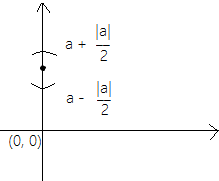
\includegraphics[width=0.2\linewidth]{list1_1.png}}
		\end{figure}
		$\{f\; |\; f(0) = 0\}\ A = \{\text{многочлены без свободного члена}\}.$\\
		\\		
		1. Докажем, что ничего, кроме функций, проходящих через $(0, 0)$, не лежит в замыкании $A.$\\		
		Рассмотрим произвольную функцию $f$, такую что $f(0) \ne 0$, и найдем ее окрестность, в которой нет точек из $A$. Без ограничения общности скажем, что $f(0) = a$, и зададим $I = (a - \frac{|a|}{2}, a + \frac{|a|}{2})$, тогда в $\sigma (0, I)$ не лежит ни одного элемента из $A$, что равносильно тому, что $f \notin \overline{A}$, что и требовалось доказать\\
		\\
		2. Докажем, что все функции проходят через $(0, 0)$ лежат в $\overline{A}$. $f$ -- произвольная функция, такая что $f(0) = 0$. Рассмотрим ее произвольную окрестность. Помимо условия в нуле у функции есть еще конечное множество точек с условием.\\		
		Тогда пусть есть $\sigma_{i}(x_{i}, I_{i})\ i = 1, ..., n$. Выберем в каждом $I_{i}$ по точке. Получим набор из $n + 1$ различной точки. Тогда составим по этим точкам интерполяционный многочлен Лагранжа. Известно, что он степени не выше $n$. $\Rightarrow$ в любой точке окрестности функции $f$ мы нашли точку из $A$. Значит, $f$ -- предельная точка $A. \Rightarrow f \in \overline{A}$. Что и требовалось доказать\\	
		\\	
		\textbf{Ответ.} Замыкание -- все функции, проходящие через (0, 0).
		
		
		
		\subsection{}
		Пусть $X$ и $Y$ -- топологические пространства, причем $Y$ хаусдорфово, и пусть $f:\ X \to Y$ -- непрерывное отображение. Докажите, что его график (т.е. множество $\Gamma_f = \{(x,f(x)):\ x \in X\}$ )
		замкнут в $X \times Y$\\
		\\
		$\blacktriangleright$\\
		Рассмотрим предельную точку графика, пусть это $(x_0, y_0)$. Предположим, что график не содержит предел $(x_0, y_0)$. Пусть $f(x_0) = y_1$, где $y_1 \ne y_0$. Тогда для $y_1, y_0$ существуют непересекающиеся окрестности.\\
		Так как отобраение непрерывно, то
		\begin{gather*}
			\forall \varepsilon\ \exists \delta:\ x_0 \in (x_0 - \delta, x_0 + \delta),\ f(x_0) \in (y_1 - \varepsilon, y_1 + \varepsilon)
		\end{gather*}
		По определению предельной точки окрестности, для любой окрестности $(x_0, y_0)$ существует хотя бы 1 точка из множества. Откуда в пересечении окрестностей еть точка из множества $\Rightarrow$ противоречие. Тогда график содержит эту предельную точку, аналогично доказывается содержание и всех остальных точек.
		\\
		\begin{comment}
			$\blacktriangleright$ Ретракт топологического пространства $X$ -- подпространство $A$ этого пространства, для которого существует непрерывное отображение $f: X \to A$, тождественное на $A:\ f(x) = x \quad \forall x \in A$.\\
			\\
			\textbf{Предложение 1}\\ Каждый ретракт в хаусдорфовом топологическом пространстве есть замкнутое множество.\\
			\\
			\textbf{Доказательство}\\ Пусть $A$ -- ретракт в хаусдорфовом топологическом пространстве $X,\ f_{\text{Id}}: X \to A$ -- ретракция. Пусть $b$ -- произвольная точка в $X$, не содержащаяся в $A$. Точки $b$ и $h(b)$ различны, так как $h(b) \in A$, $b \not \in A$. Выберем окрестность $U_{1}$ точки $b$ и окрестность $V$ точки $h(b)$ так, чтобы $U_{1} \cap V = \varnothing$, -- это возможно, так как подмножество хаусдорфова топологического пространства -- также топологическое пространство, а значит, такие окрестности существуют по определению.\\
			\\
			Возьмем $U_{2}$ точки $b$, такую что $h(U_{2}) \subset V$ -- это возможно в силу непрерывности $f$. Пусть $U = U_{1} \cap U_{2}$. Для U также верны свойства $U_{1}, U_{2}\!\!:\ U \cap V = \varnothing,\ f(U) \subset V$. Из этого делаем вывод, что $\forall x \in U \quad h(x) \neq x$. Это значит, что $U \cap A = \varnothing$. Таким образом, $b$ обладает окрестностью, не пересекающейся с $A$. Значит, $b$ не является предельной точкой $A$ и все предельные точки $A$ содержатся в $A$. Что и требовалось доказать. Что и требовалось доказать.\\ 
			\\
			\textbf{Предложение 2}\\ Подмножество $A$ топологического пространства $X$ -- ретракт $\Leftrightarrow$ всякое непрерывное отображение $A \to Y$ продолжается до непрерывного $X \to Y \quad \forall Y.$\\
			\\
			\textbf{Доказательство}\\ Пусть $g_{\text{Id}}:\ X \to A$ -- ретракция, $f: A \to Y$ -- непрерывное отображение. Тогда $f \circ g$ -- непрерывное продолжение отображения $f$ на все $X$. Теперь пусть всякое непрерывное отображение $A \to Y$ продолжается до непрерывного на все $X$. Тогда и тождественное отображение $A \to A$ обладает таким продолжением, которое и будет ретракцией $X \to A$. Что и требовалось доказать.\\
			\\
			Теперь вернемся к задаче. Требуется доказать, что $\Gamma$ -- ретракт в $X \times Y$. Рассмотрим непрерывное отображение $\varphi:\ \Gamma \to Z$. Тогда композиция $g = \phi \circ h_{f} \circ p:\ X \times Y \to Z$, где $h_{f}: X \to$ $\Gamma$ -- гомеоморфизм $(x \mapsto f(x)) \Rightarrow$ взаимнооднозначно, компоненты отображения $h_{f}$ -- непрерывные отображения $\text{Id}: X \to X, \quad y = f(x) \Rightarrow h_{f}$ непрерывно, $h^{-1}_{f}:\ F \to X$ -- сужение проекции $p: X \times Y \to X$, на подпространстве $\Gamma$ совпадает с $\varphi. \quad \blacktriangleleft$\\
		\end{comment}
		
		
		
		\subsection{}
		Пусть $A$ и $B$ -- замкнутые подмножества топологического пространства $X$, причем $A \cup B$ и $A \cap B$ связны. Докажите, что $A$ и $B$ связны. Верно ли это, если не требовать замкнутости $A$ и $B?$\\
		\\
		$\blacktriangleright$\\
		Докажем от противного:\\
		Пусть $A$ несвязно, тогда $A = A_1 \cup A_2$, где $A_1, A_2$ непустые и замкнутые множества.\\
		1) $A_1 \cap B \ne \varnothing$ и $A_2 \cap B \ne \varnothing$\\
		Тогда рассмотрим $(A_1 \cup A_2) \cap B = (A_1 \cap B) \cup (A_2 \cap B) = A \cup B$ -- связно по условию. Тогда $(A_1 \cap B),\ (A_2 \cap B)$ замкнуты (как пересечения замкнутых), откуда связное множество разбито на два непересекающихся замкнутых подмножества.\\
		\\
		2) $A_1 \cap B \ne \varnothing$ и $A_2 \cap B = \varnothing$\\
		$(A_1 \cup A_2) \cup B = A_2 \cup (A_1 \cup B)$ тогда $(A_1 \cup B)$ и $A_2$ замкнуты\\
		\\
		3) $A_1 \cap B = \varnothing$ и $A_2 \cap B = \varnothing$\\
		не может быть, так как $A \cup B$ связно\\
		\\
		В случае когда $A$ и$\slash$или $B$ незамкнуто, есть контрпример: $A = [1, 2],\ B = \left[0, 1\right) \cup \left[2, 3\right]$, $A \cap B = \{2\}$ и $A \cup B = [0, 3]$\\
		
		\begin{comment}
		По условию $A \cup B$ связно, тогда либо $A_1 \supset A \cap B$, либо $A_2 \supset A \cap B$. Без ограничения общности $A_1 \supset A \cap B$, тогда $A_2$ и $A_1 \cap B$ разбивают $A \cap B$ на 2 непустых замкнутых множества. $A_1, A_2$ замкнуты в $A \cap B$, так как замкнутое подмножество замкнутого множества замкнуто в объемлющем пространстве $\Rightarrow$ противоречие со связностью $A \cup B$, тогда $A$ связно, аналогично для $B$\\
		
		\\
		
			\textbf{Связное множество топологического пространства} -- множество, которое нельзя разбить на два непересекающихся открытых множества. Также для $A$ и $B$ и индуцированной топологии на них эквивалентны определения, что $A$ и $B$ нельзя разбить на два непересекающихся замкнутых множества, так как $A$ и $B$ при разбиении на два множества являются дополнениями друг к другу, а значит, являются и открытыми и замкнутыми одновременно. Замкнутые множества в $A$ замкнуты в $X$, так как они получены путем пересечения $A$ -- замкнутого в $X$, -- с другими замкнутыми.\\
			\\
			Аналогично для $B,\ A \cap B,\ A \cup B.$\\		
			$A$ и $B$ замкнуты, $(X, \tau)$ -- топологическое пространство. $A \cup B, A \cap B$ -- связны.\\		
			\textbf{1. Доказать: $A, B$ -- связны.} Докажем от противного (для $A, B$ эквивалентно).\\		
			Пусть $A$ -- несвязно. Тогда разобьем $A$ на два непересекающихся замкнутых (также являющихся открытыми) множества. $A = C \cup D$ -- замкнуто.\\		
			\begin{figure}[h]
			\center{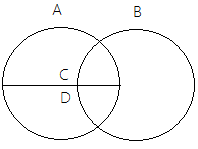
\includegraphics[width=0.2\linewidth]{list1_2.png}}
			\end{figure}
			1) $(C \cap B \neq \varnothing) \cap (D \cap B \neq \varnothing)$\\		
			Рассмотрим $(C \cap B) \cup (D \cap B) = A \cap B$ -- связано, но $C \cap B$, где $C$ -- замкнуто, $B$ -- замкнуто, также замкнуто, $D \cap B$ -- замкнуто.\\		
			Мы разбили связное множество на два непересекающихся замкнутных множества. Невозможно.\\
			\\
			2) $C \cap B = \varnothing$\\		
			Рассмотрим $C \cap (D \cap B) = A \cap B$ -- связно, но $C$ -- замкнуто в индуцированной топологии на $A \cap B$, $D \cap B$ замкнуто $\Rightarrow$ мы разбили связное множество $A \cap B$ на два непересекающихся замкнутых множества. Невозможно. Что и требовалось доказать Аналогично с $B.$\\
			\\
			\textbf{2. Верно ли это, если не требовать замкнутости $A$ и $B$? }\\
			\\		
			Определим топологию на $\mathbb{R}$, порожденную евклидовой метрикой. $A = \{0\},\ B = (-1, 0) \cap (0, 1)$ -- открыто и несвязно.\\		
			$A \cap B = \varnothing$ -- связно.\\		
			$A \cup B = (-1, 1)$ -- связно.\\
			\\
			\textbf{Ответ.} Нет. 
		\end{comment}
	
	
	
		\subsection{}
		Пусть $X, Y, Z$ -- топологические пространства, причем $Y$ компактно, и пусть $f: X \times Y \to Z$ -- непрерывное отображение.\\
		Докажите, что для любого открытого множества $W \subset Z$ множество $M = \{x \in X\ \forall y \in Y:\ f(x,y) \in W\}$ открыто в $X$.\\
		\\
		$\blacktriangleright$\\
		$x_0 \in M$ $\forall y_i:\ f(x_0, y_i) \in W$\\
		Так как $Y$ -- компактен, то для окретсностей $y_i$, назовем их $U_i$, выполнено: $\exists n: U_1 \cup U_2 \cup \ldots \cup U_n \supset Y_{}$.\\
		Рассмотрим окрестность $(x_0, y_i):\ V_i$ так как $f$ непрерывно, $W$ открыто, то $f(V_i) \subset W$\\
		$V_i = S_i \times U_i$, где $S_i$ -- окрестность $x_i$ и $S = S_1 \cap S_2 \cap \ldots \cap S_n$, так как $S_1 \cap \ldots \cap S_n$ -- пересечение конечного числа открытых множеств, то $S_{}$ открыто.\\
		Тогда $(x_0, y) \in (S_{}, U_{})$, тогда заметим, что $f(S_{}, U_{}) \subset W$ (по построению), тогда множество из $(x_0, y)$ -- открыто, откуда открыто и $M$, что и требовалось.
		\begin{comment}
		По условию: $\forall$ открытого $W \subset Z: \quad M = \{ x \in X\ \forall y \in Y:\ f(x,y) \in W \}$ открыт в $X$\\
		\begin{enumerate}
		\item
		Рассмотрим $x_0 \in M$\\
		$\forall y_i\ \exists V = V_{\tau} \times V_i^{\prime}$\\
		$(x_0, y_i) \in V_i^{\prime}$\\
		$f(x_0, y_i) \in W$
		
		\item
		Так как $Y$-компакт,\\
		то  $\exists n: V_1^{\prime} \cup V_2^{\prime} \cup \ldots \cup V_n^{\prime} \supset Y$\\
		Где $V_i^{\prime}$ открытое множество\\
		Из (1):
		\begin{gather*}
		V_1^{\prime} \to V_1\\
		V_2^{\prime} \to V_2\\
		\ldots\\
		V_n^{\prime} \to V_n
		\end{gather*}
		Тогда $U = V_1 \cap V_2 \cap \ldots \cap V_n$ -- открыто и конечно(как пересечение конечного числа откртых множеств), а также $x_0 \subset U$\\
		
		\item 
		$(x_0, y_i) \subset U \times Y \subset U \times (V_1 \cup V_n)$\\
		$f(U \times Y) \subset W$ (по построению)\\
		Тогда $U \subset M$ открыто\\
		Откуда $\forall x_0 \in M\ \exists U_0: x \in U_0$ и $U_0$ открыто,\\
		Следовательно $M$ -- открыто
		\end{enumerate}
		\end{comment}
		